% %
% LAYOUT_E.TEX - Short description of REFMAN.CLS
%                                       99-03-20
%
%  Updated for REFMAN.CLS (LaTeX2e)
%
% Preamble
\documentclass[twoside,a4paper]{refart}
% importing packages
\usepackage{makeidx}
\usepackage{ifthen}
\usepackage{url}
\usepackage{csquotes}
\usepackage{graphicx}
\usepackage{float}
\usepackage{caption}
\usepackage{hyperref}
\usepackage{titlesec}
\usepackage{todonotes}
\usepackage{subcaption}
\usepackage{xcolor}
\usepackage{nameref}
\usepackage{listings}
\usepackage{verbatim}
\usepackage[T1]{fontenc}

% Setting up document
\def\bs{\char'134 } % backslash in \tt font.
\newcommand{\ie}{i.\,e.,}
\newcommand{\eg}{e.\,g..}
\DeclareRobustCommand\cs[1]{\texttt{\char`\\#1}}
\captionsetup{hypcap=false}
% Minipage spacing
\def\bmp{\begin{minipage}{0.48\linewidth}\small} 
\def\emp{\end{minipage}\smallskip}

\title{\LaTeX\ Guide Guide}
\author{
John Pan (jpthek9@gmail.com)\\
\url{https://github.com/SnpM}
}

\date{\url{https://github.com/SnpM/latex-guide-guide.git}\\\today}
\emergencystretch1em  %

\pagestyle{myfootings}
\markboth{\LaTeX\ Guide Guide}%
         {\LaTeX\ Guide Guide}

\makeindex 

\setcounter{tocdepth}{2}

\begin{document}

\maketitle

\begin{abstract}
         \LaTeX\ is a high-quality typesetting standard for academic and professional documents. The system may seem complicated because of its coding syntax, but powerful \LaTeX\ editors such as Overleaf streamline the learning the process. A wealth of high-quality \LaTeX\ templates exist online, enabling authors to focus on content rather than appearance. This guide teaches new \LaTeX\ users how to author an instructional \LaTeX\ document in Overleaf based on the \texttt{refman} template.
\end{abstract}

The \LaTeX\ Guide Guide is part of my final project for the Technical Communication course at Thomas Edison State University, mentored by Dr. Douglas Hoehn. 

\tableofcontents

\newpage


%%%%%%%%%%%%%%%%%%%%%%%%%%%%%%%%%%%%%%%%%%%%%%%%%%%%%%%%%%%%%%%%%%%%
% \newpage after every \section
\newcommand{\sectionbreak}{\clearpage}

\section{Introduction}\label{sec:Introduction}


{\subsection{What is \LaTeX?}
LaTeX (pronounced \enquote{Lay-Tech}) is a document preparation system for technical and scientific documents. LaTeX is not a word processor; instead, it encourages authors to focus on content rather than the appearance of their documents. LaTeX is great for producing formatted documents in academic, scientific, and professional contexts\footnote{See https://www.latex-project.org/about/}.
\par


\subsection{Authoring with \LaTeX}
Authoring projects with \LaTeX\ is streamlined with the many tools and templates available online.\\
Overleaf is a beautiful web-based LateX editor designed for collaboration; it boasts 3.9 million plus users from over 3,600 different institutions\footnote{Official Overleaf website: https://www.overleaf.com/about}
\par
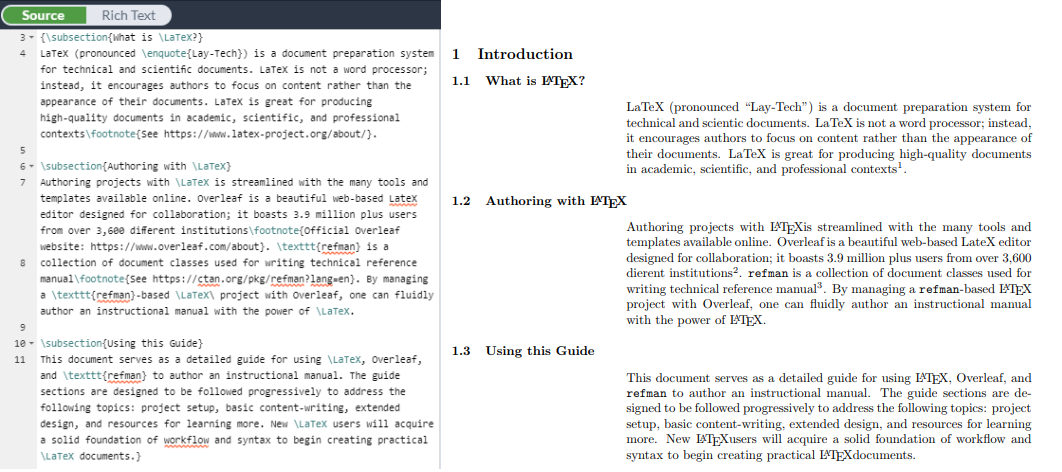
\includegraphics[width=\linewidth]{graphics/IntroSource.png}
\par
\texttt{refman} is a collection of document classes used for writing technical reference manual\footnote{See https://ctan.org/pkg/refman?lang=en}. By managing \texttt{refman}-based projects with Overleaf, authors can fluidly create instructional manuals with the power of \LaTeX.

\subsection{Using this Guide}
This document serves as a detailed guide for using \LaTeX, Overleaf, and \texttt{refman} to author an instructional manual. The guide sections are designed to be followed progressively to address the following topics: project setup, basic content-writing, extended design, and resources for learning more. New \LaTeX\ users will acquire a solid foundation of workflow and syntax to begin creating practical \LaTeX\ documents.}

\section{Getting Started}\label{sec:Getting Started}

The Getting Started section explains how to register with Overleaf, create a new project based on the \texttt{refman} template, then use Overleaf's editor interface to configure the project.

\subsection{Register}
Web access to Overleaf will be required throughout this guide. Ensure you have an Overleaf account by registering at \url{https://www.overleaf.com/register}. 

\begin{minipage}{\linewidth}
\fbox{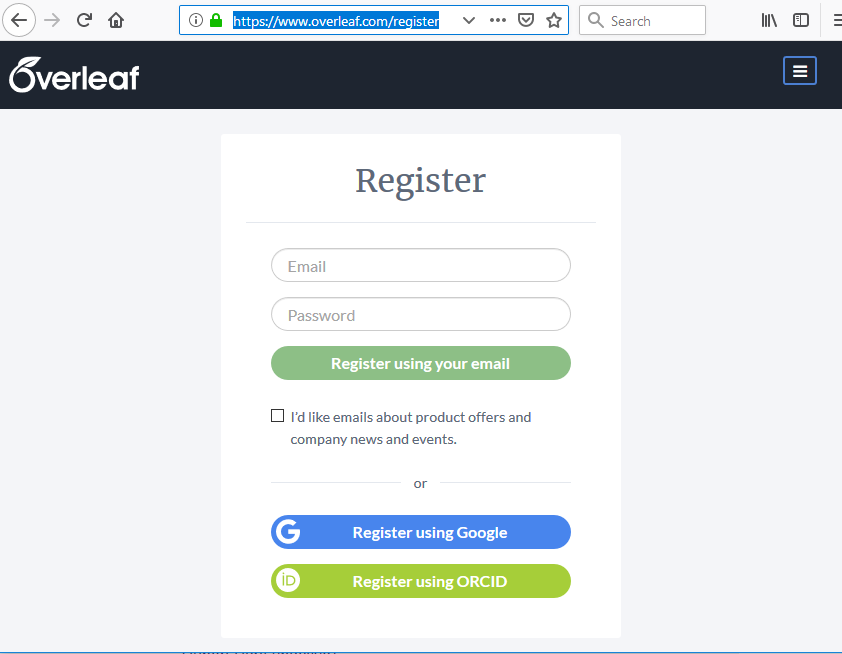
\includegraphics[width=\linewidth]{graphics/RegisterOverleaf.PNG}}
\captionof{figure}{Overleaf registration site \texttt{refman}}
\end{minipage}

Registering will give you access to Overleaf's powerful features including file management, cloud storage, and change tracking.

\subsection{New Project}
Navigate to
\url{https://www.overleaf.com/latex/templates/refman-format-technical-reference-manuals/jjrfdfpyxzvz} to start a new project with the \texttt{refman} template.

\begin{minipage}{\linewidth}
\centering
\fbox{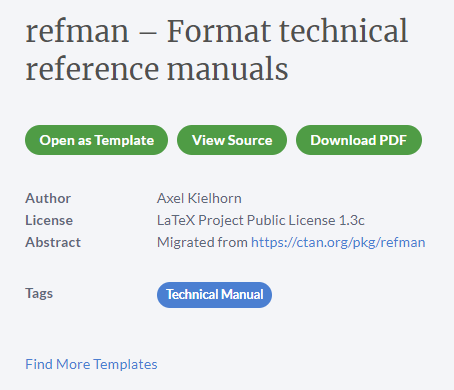
\includegraphics[width=.5\linewidth]{graphics/RefmanTemplate.PNG}}
\captionof{figure}{Overleaf registration site \texttt{refman}}
\end{minipage}

Click the 'Open as Template' button to create a new project based on the template; this will open the editor interface for the new project.

\begin{minipage}{\linewidth}
\fbox{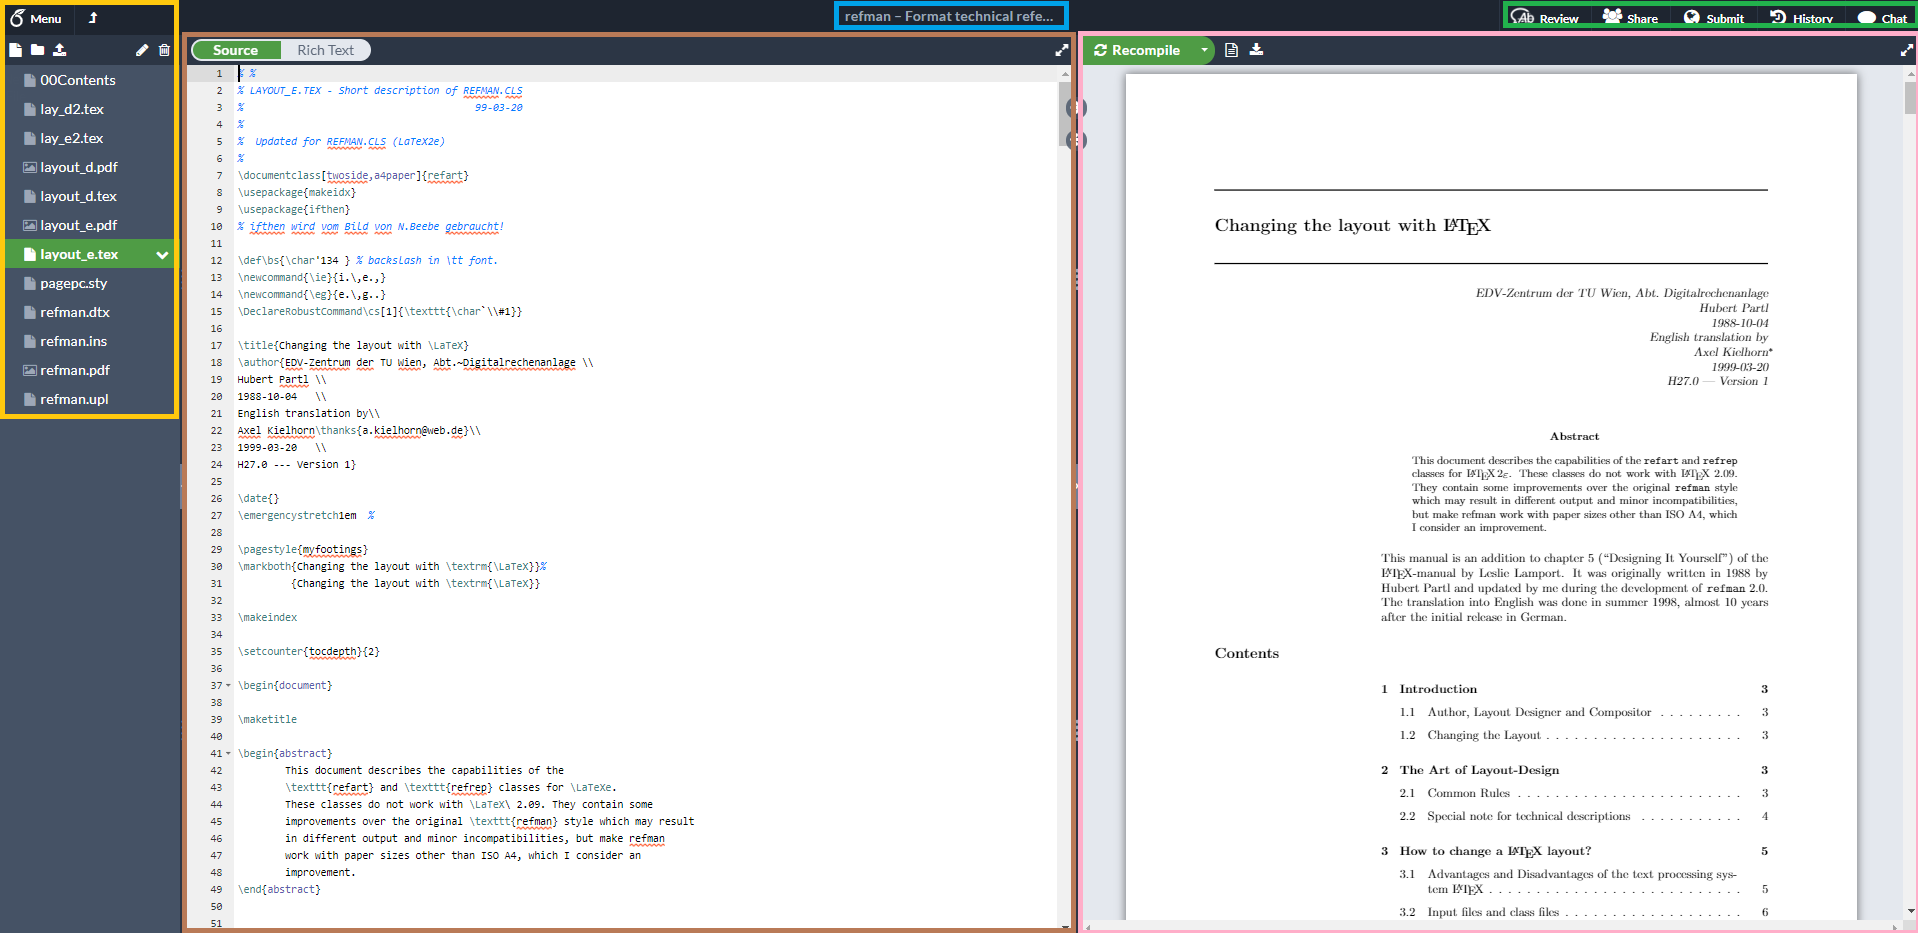
\includegraphics[width=\linewidth]{graphics/OverleafEditorInterface.PNG}}
\captionof{figure}{Overleaf Editor Interface}
\label{fig:EditorInterface}
\end{minipage}

The editor interface contains five interactable areas:
\begin{enumerate}
    \item \fcolorbox{black}{yellow}{Gold} left sidebar - File and project management
    \item \fcolorbox{black}{brown}{Brown} left textbox - \LaTeX\ document source editing
   \item \fcolorbox{black}{pink}{Pink} right textbox - Compiled \LaTeX\ document view
    \item \fcolorbox{black}{cyan}{blue} top-center title box - Modify title of Overleaf project
    \item \fcolorbox{black}{green}{Green} top-right button group - Change tracking and other collaboration tools
\end{enumerate}
See \url{https://www.overleaf.com/learn/latex/Tutorials} for comprehensive tutorials about the Overleaf web interface.

\subsection{Configuring Project}
The 'Title' and 'Main Document' of the project can now be configured.
\par
Highlight the top-center \textit{title box} to edit the project title (blue area in figure \ref{fig:EditorInterface}).

\begin{minipage}{\linewidth}
\fbox{
\includegraphics[width=\linewidth]{graphics/Rename.PNG}}
\captionof{figure}{Rename project title}
\end{minipage}

Locate and click the pencil symbol then enter your desired project name.

Now navigate to the left \textit{project management sidebar} (gold area in figure \ref{fig:EditorInterface}). Click the 'Menu' button in the top-left to open the \textit{project  settings window}.

\begin{minipage}{\linewidth}
\centering
\fbox{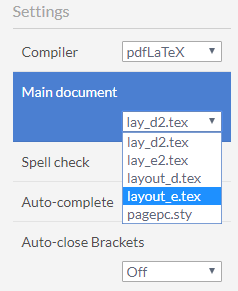
\includegraphics[width=.5\linewidth]{graphics/MainDocument.PNG}}
\captionof{figure}{Project Settings; Configuring main document}
\end{minipage}

Set the 'Main document' to the \path{layout_e.tex} document to compile \path{latex_e.tex} as the main document.
\par
The project is now configured and ready for adding content. See section \ref{sec:Basic Writing} to begin writing your \LaTeX\ project.

\section{Basic Writing}\label{sec:Basic Writing}
This section introduces basic \LaTeX\ syntax. Learn how to configure the project Preamble then write your first section in \LaTeX\ code!
\subsection{Basic LaTeX}
Authoring with \LaTeX\ is similar to writing a program: type code to define program behavior, compile program into consumable file, then open file and enjoy! There are four key principles to consider when authoring documents with \LaTeX:
\begin{enumerate}
    \item Content is written in plaintext.
    \item Formatting and features are applied with commands.
    \item Packages provide extra text, graphics, and presentation commands.
    \item \LaTeX\ code is typically compiled into a read-only professional-looking PDF.
\end{enumerate}
With these principles in mind, let's start learning some basic \LaTeX\ syntax and commands\footnote{Based on existing instructional material: http://www.rpi.edu/dept/arc/training/latex/class-slides-pc.pdf}.
%TODO: Cite this
\par
The \verb|"\"| backslash character is used to begin all \LaTeX\ commands. E.g.
\verb|\LaTeX| compiles to \LaTeX.
\par
Some commands take input enclosed in curly braces. E.g.\\
\verb|\textit{This text is italicized}| $\rightarrow$ \textit{This text is italicized}.
\par
{\large\textbf{Common commands include:}}\\
\verb|\\|, \verb|\newline|, \verb|\par|\\
Various ways to generate new lines.
\par
\verb|\newpage|\\
Insert page break to start text on new page.
\par
\verb|\textit{text}|, \verb|\textbf{text}|, \verb|\texttt{text}|\\
Modifies text to be \textit{italicized}, \textbf{bold}, or \texttt{scientific}.
\par
\verb|\usepackage{<packageName>}|\\
Define a \LaTeX\ package to use for modular commands and behaviors in your project.
\par
\verb|\chapter{<title>}|, \verb|\section{<title>}|, \verb|\subsection{<title>}|\\
Mark the beginning of new chapters/sections/subsections.
\par
\verb|\title{<document title>}|, \verb|\author{<author>}|, \verb|\date{<date>}|\\
Define the document's title, author, and date.
\par
\verb|\maketitle|\\
Print the document's title, author, and date.
\par
\verb|\markboth{left title}{right title}|\\
Defines the headings or footings on either side of the page.
\par
\verb|\url{<website link>}|\\
Prints a clickable website link on the page.
\par
\verb|\today|\\
Print today's date.
\par
{\large\textbf{Certain characters have special meanings in \LaTeX.}}\\
\begin{tabular}{r|l}
\textbf{Char} & \textbf{Meaning} \\
\verb|%|& Parameter in a macro; also used in tables \\ 
\verb|$|& Used to begin and end math mode \\
\verb|%|& Used for comments in the source file \\
\verb|&|& Tab mark, used in alignments and tables \\
\end{tabular}
\par

{\large\textbf{Environments are uniquely formatted blocks of text}}\\
Environments define blocks of texts that receive special formatting or processing. They are delimited by the \verb|\begin{<type>}| and \verb|\end{<type>}| commands that take . Everything between \verb|\begin| and \verb|\end| will be processed based on the environment <type> inputted.
\par
For now, you only need knowledge about the \texttt{document} and \texttt{abstract} environment types:\\
\begin{itemize}
\item\verb|\begin{document}| and \verb|\end{document}|\\
Define area for all document text. Everything included inside the \verb|begin{document}| \verb|\end{document}| commands will be rendered in the final document.

\item\verb|\begin{abstract}| and \verb|\end{abstract}|\\
Define area for the abstract of the document. The abstract is uniquely formatted by the template to give readers a quick summary about the document.

\item\verb|\begin{minipage}{<width>}| and \verb|\end{minipage}|\\
Define area for minipage. Minipages are useful for containing graphics and other contents in a single paragraph box.
\end{itemize}

\par
To learn more about environments, see Overleaf's tutorial at \url{https://www.overleaf.com/learn/latex/Environments}.\\
For a comprehensive guide about \LaTeX\ syntax and commands, see \url{https://www.rpi.edu/dept/arc/docs/latex/latex-intro.pdf}.\\
To learn more about \LaTeX\ document structure, see \url{https://www.overleaf.com/learn/latex/Creating_a_document_in_LaTeX}.
\par
In the next subsection, you will use basic knowledge of \LaTeX\ to configure the \texttt{preamble} of your project.

\subsection{Preamble and Abstract}
We previously set the \texttt{Main Document} of the project in Overleaf to
\path{layout_e.tex}. Locate this file and open it to begin editing the \texttt{preamble}.

\begin{minipage}{\linewidth}
\centering
\fbox{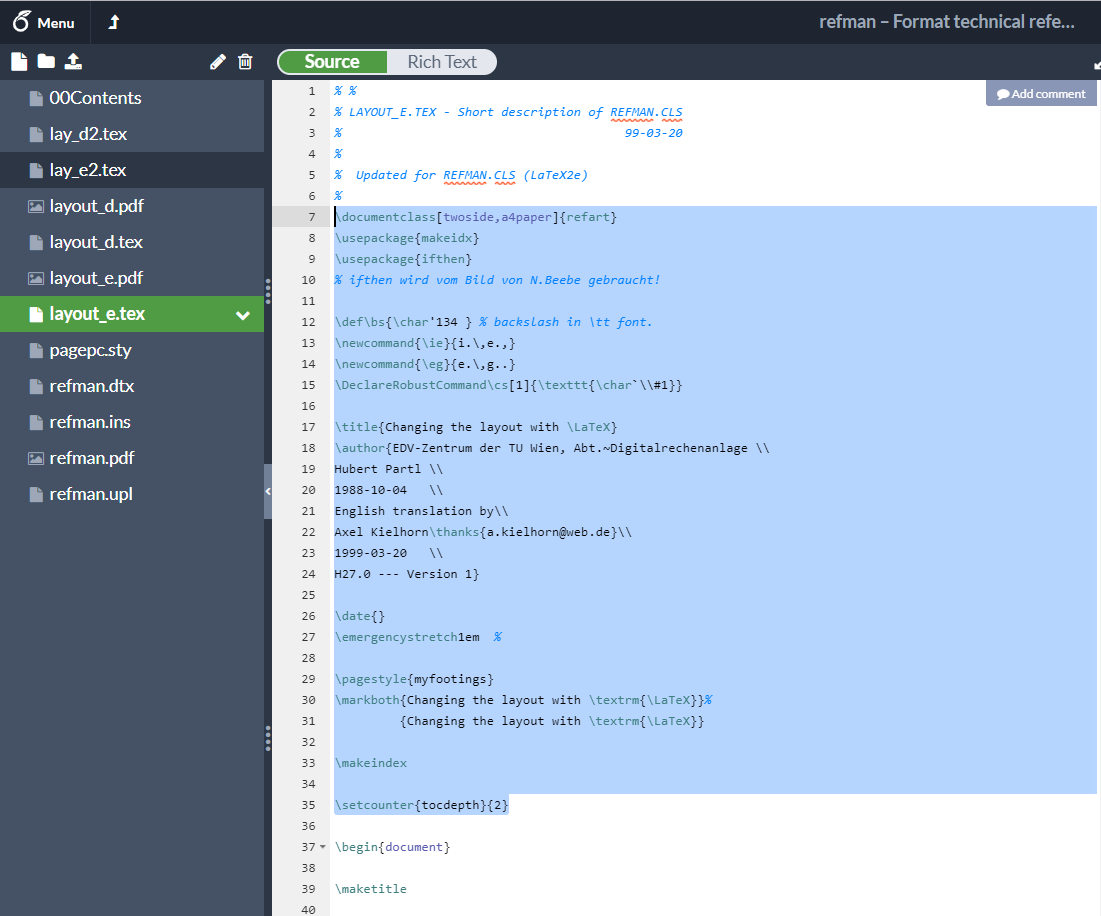
\includegraphics[width=\linewidth]{graphics/MainDocumentPreamble.PNG}}
\captionof{figure}{Locating \detokenize{layout_e.tex file}}
\label{fig:Preamble}
\end{minipage}

Notice the highlighted section in figure \ref{fig:Preamble}. The area of from the start of the document to the \verb|\begin{document}| command is called the \texttt{preamble}: the first part the main document where you describe the title, packages used, and more information about the document. Configuring the \texttt{preamble} is necessary to customize the \LaTeX\ project for your project's requirements.

    \subsubsection{Adding Packages}
First, extend the available commands in your \LaTeX\ project. Locate the \verb|\usepackage{ifthen}| command around \texttt{line 9}. Copy-paste the following commands after that line to start writing with several useful packages:
\par
\begin{minipage}{\linewidth}
\begin{verbatim}
\usepackage{url} %Clickable URLs
\usepackage{csquotes} %Advanced quotations
\usepackage{graphicx} %Add graphics
\usepackage{caption} %Captioning for figures
\usepackage{xcolor} %Change text color
\usepackage{nameref} %Reference labels by name
\usepackage{titlesec} %Modify sectioning behavior
\usepackage[T1]{fontenc} %Change font encoding
\usepackage{verbatim} %Print text verbatim
\end{verbatim}
\end{minipage}
\par
We will explore some commands in these packages in the later \nameref{sec:Extended Writing} section.\\

    \subsubsection{Title, Author, and Date}
Configure the heading information of the document by modifying input in the \verb|\title|, \verb|\author|, and \verb|\date| commands. For example, locate the \verb|\title| command and customize the input to whatever you want:
\par
\textbf{Original:}\\
\verb|\title{Changing the layout with \LaTeX}|
\par
\textbf{Modified:}\\
\verb|\title{Overleaf Guide Guide :D}|
\par
Similarly, configure the \texttt{author} and \texttt{date} of the document by change the text inside the curly brackets. Use \verb|\\| for creating new lines in text.
\par
\begin{minipage}{\linewidth}
\begin{verbatim}
\author{
    John Pan (jpthek9@gmail.com)\\
    \url{https://github.com/SnpM}\\
    John likes Ed Sheeran.
}
\end{verbatim}
\end{minipage}
\par
...
\par
\begin{minipage}{\linewidth}
\begin{verbatim}
\date{
    \url{https://github.com/SnpM/latex-guide-guide.git}\\
    \today\\
    Today is National Pet Day.
}
\end{verbatim}
\end{minipage}
\par



    
\subsection{Adding Content}
   Now that the preamble is set up and you're more familiar with \LaTeX\, it's time to begin writing content for the document. This subsection details how to modify the \textit{Abstract} and individual sections of the document.
    
    \subsubsection{Modifying Abstract}    
    The \textit{abstract} of the document is one of the first parts of the document environment; it is a block of text specially formatted for delivery of the document's purpose to readers. The abstract is defined within the \verb|begin{abstract}| and \verb|\end{abstract}| \textit{environment}. To modify the document's abstract, locate and edit the text after the \verb|\begin{abstract}| command. Try to experiment with different font faces and other \LaTeX\ commands such as \verb|\url{<website link>}|.
    
    \begin{minipage}{\linewidth}
        \centering
        \fbox{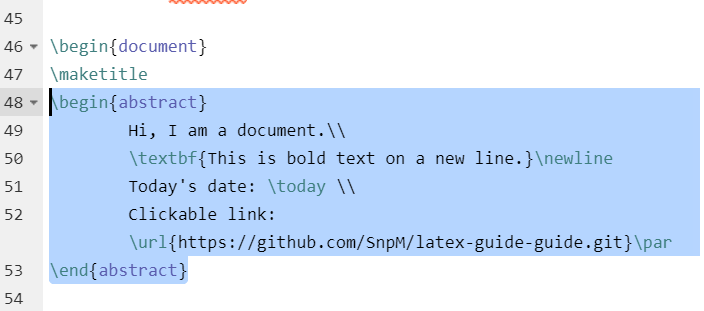
\includegraphics[width=.95\linewidth]{graphics/Abstract.PNG}}
        \captionof{figure}{Source for customized abstract}
        \label{fig:Preamble}
    \end{minipage}
 
    \subsection{Modifying Sections}
    Sections are different from the \textit{abstract} because they are not defined with environments (\verb|\begin ... \end|). Instead, sections are defined with a single command indicating the start of the section. The section automatically continues until another section is defined or the document ends.
    \par
    Navigate to the first section identified by the first \verb|\section| command.
    \begin{minipage}{\linewidth}
        \centering
        \fbox{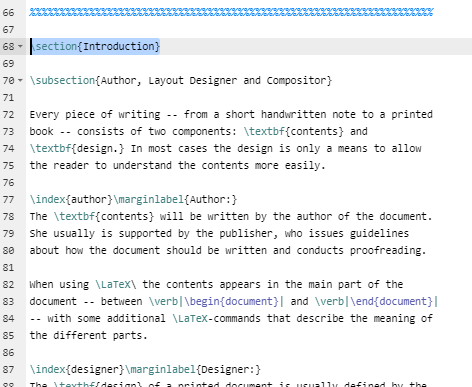
\includegraphics[width=.95\linewidth]{graphics/FirstSection.PNG}}
        \captionof{figure}{The first section is titled \textit{Introduction}}
        \label{fig:Preamble}
    \end{minipage}
    
    

\section{Extended Writing}\label{sec:Extended Writing}
More advanced features
\subsection{Modularize Project}
\subsection{Add Graphics}\label{subsec:AddGraphics}
\subsection{Add References}
\subsection{Advanced Formatting}

\section {Resources}\label{sec:Resources}
Stuff about online resources.
\subsection{Templates}
\subsection{Further Learning}

%%%%%%%%%%%%%%%%%%%%%%%%%%%%%%%%%%%%%%%%%%%%%%%%%%%%%%%%%%%%%%%%%%%%%%

\input lay_e2

%%%%%%%%%%%%%%%%%%%%%%%%%%%%%%%%%%%%%%%%%%%%%%%%%%%%%%%%%%%%%%%%%%%%%%

\printindex

\end{document}
